\jxhj{%教学后记
	}
\skrq{%授课日期
	2017年12月19日 4-5节}
\ktmq{%课题名称
	 倒角与倒圆角}
\jxmb{%教学目标,每行前面要加 \item
	\item 掌握FANUC上的倒角与拐圆角指令;
	\item 掌握Siemens上的倒角与拐圆角;
	\item 掌握倒角与拐圆角编程。
}
\jxzd{%教学重点,每行前面要加 \item
	\item 掌握FANUC上的倒角与拐圆角指令;
	\item 掌握Siemens上的倒角与拐圆角。 }
\jxnd{%教学难点,每行前面要加 \item
	\item 掌握倒角与拐圆角编程。 }
\jjff{%教学方法
	通过讲述、举例、演示法来说明;}

\makeshouye %制作教案首页

%%%%教学内容
\subsection{组织教学}
\begin{enumerate}[\hspace{2em}1、]
	\item 集中学生注意力;
	\item 清查学生人数;
	\item 维持课堂纪律;
\end{enumerate}

\subsection{复习导入及主要内容}
\begin{enumerate}[1、]
\item 加工中心概述;
\item Fanuc加工中心换刀;
\item Fanuc数铣换刀;
\item 编程实例。
\end{enumerate}

\subsection{教学内容及过程}

倒角及倒圆角是数控铣削、加工中心中常见的结构,利用数控系统中的倒圆角,倒角指令可以使程序的编制简化。
\begin{figure}[h]
	\centering
	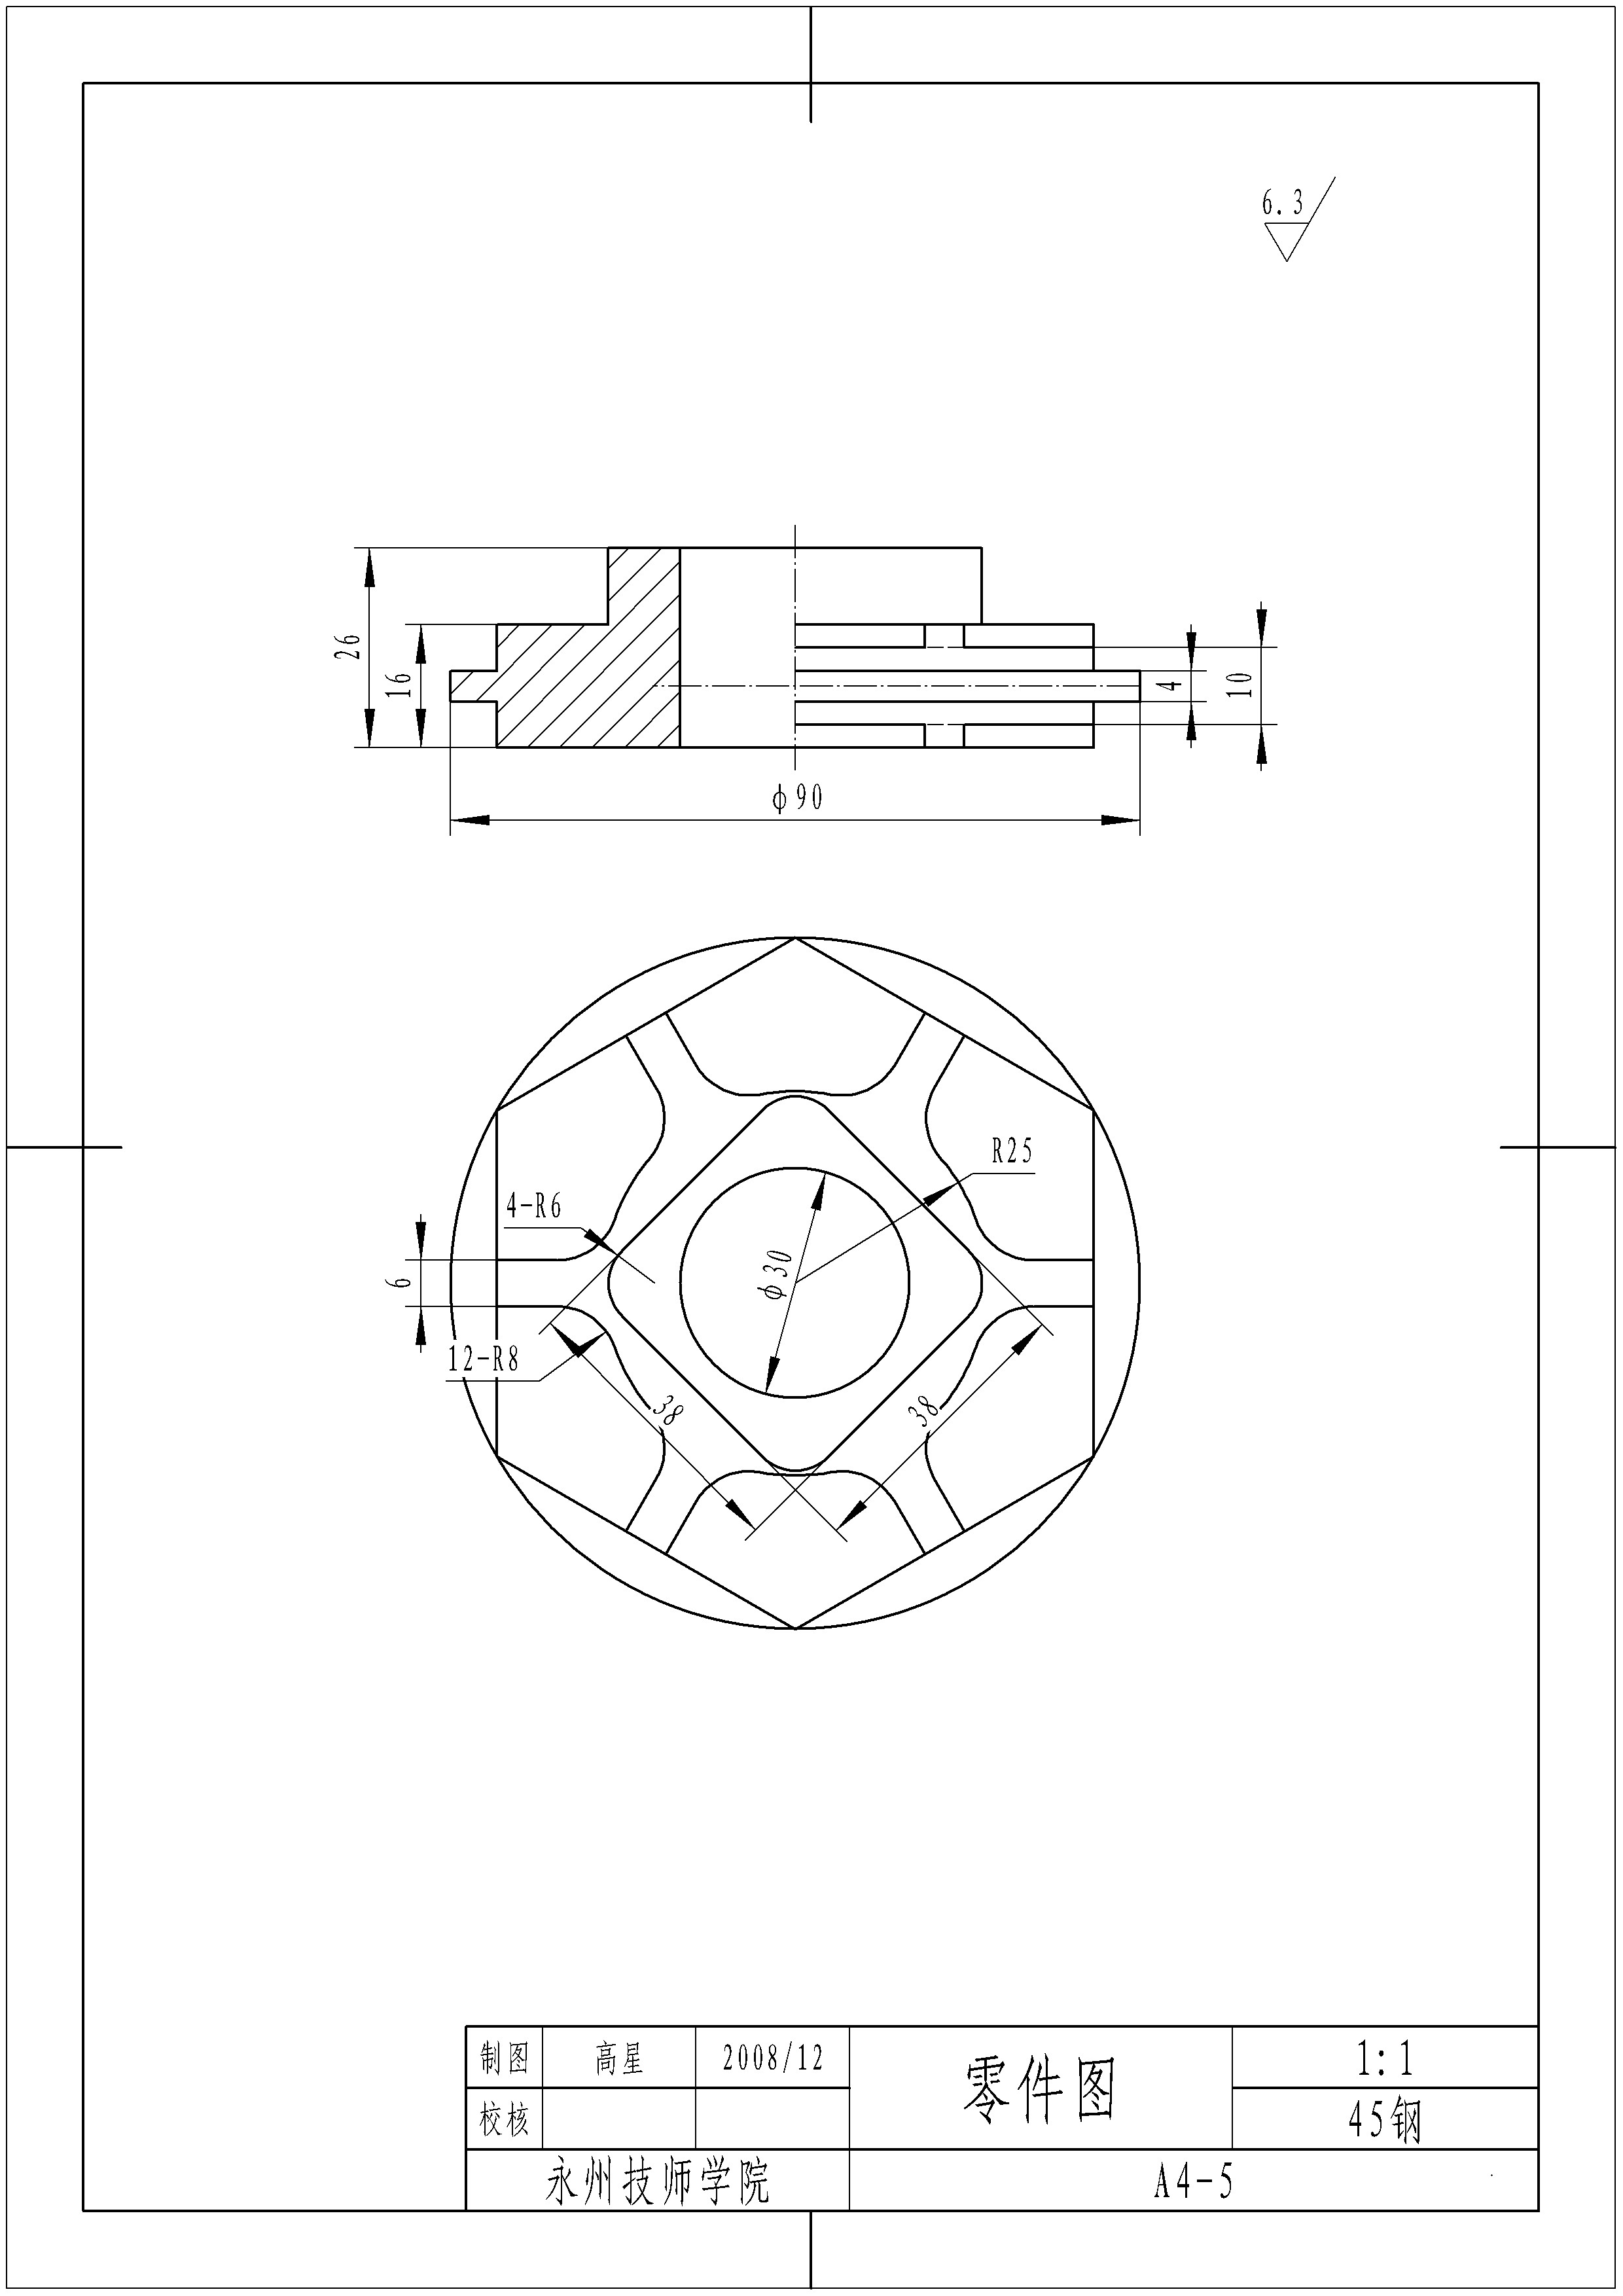
\includegraphics[width=0.8\linewidth,trim=100 200 100  200,clip]{data/image/28-1}
	\caption{示例}
	\label{fig:28-1}
\end{figure}

\begin{figure}[h]
	\centering
	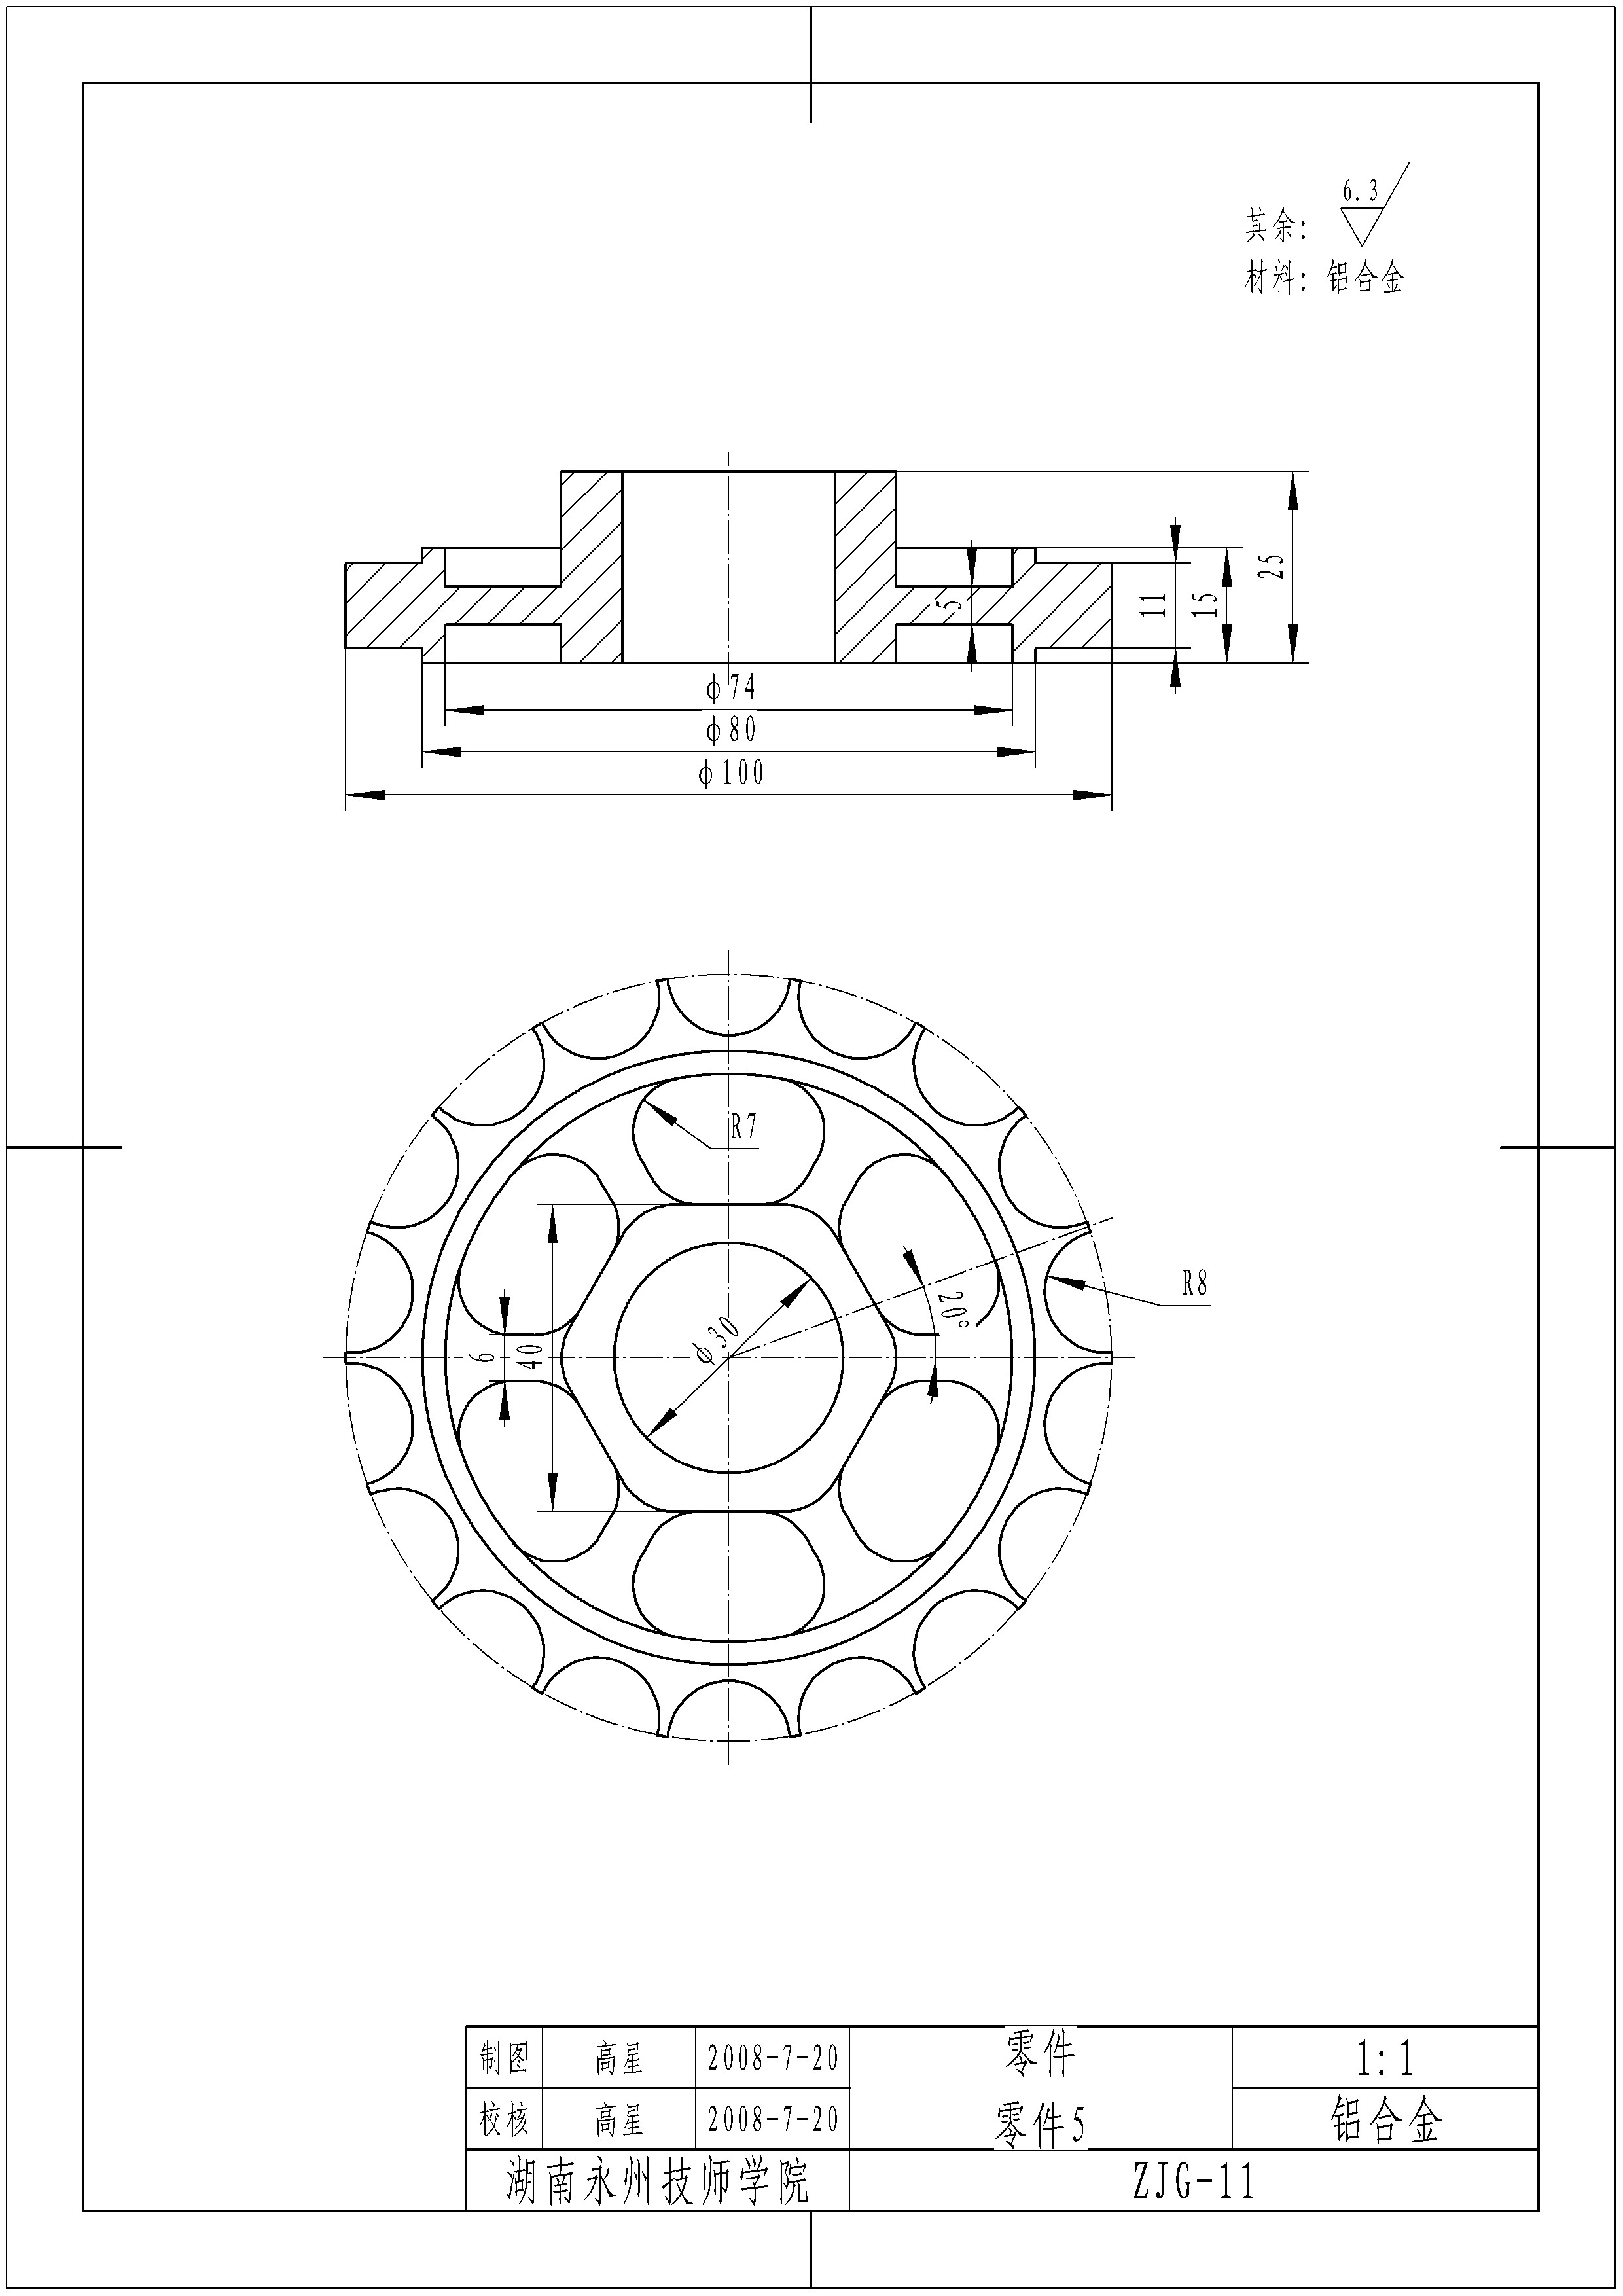
\includegraphics[width=0.8\linewidth,trim=100 200 100  150,clip]{data/image/28-2}
	\caption{示例}
	\label{fig:28-2}
\end{figure}

\subsubsection{Fanuc上的倒角、倒圆角的指令格式}
	
1、在直线插补G1或圆弧插补G2、G3程序段的末尾,加上倒角或倒圆角的指令:

……,C\_\_\_\_;(倒角)

……,R\_\_\_\_;(倒圆角)

2、可以用在以下的程序段之间:

在直线插补和直线插补程序段之间

在直线插补和圆弧插补程序段之间

在圆弧插补和直线插补程序段之间

在圆弧插补和圆弧插补程序段之间

3、应用条件:

直线与直线、直线与圆弧、圆弧与圆弧要有虚拟交点

虚拟交点坐标已知或方便求出

因为编程时,直线插补、圆弧插补的目标点必须是它们的虚拟交点。

4、说明:

A、倒角和拐角圆弧过渡只能在G17、G18、G19指定的平面内执行。

B、指定倒角或拐圆角过渡的程序段的下一个程序段必须跟随一个用直线插补G1或圆弧插补G2、G3指令的程序段,如果下一个程序段不包含这些指令,系统会出现报警。

C、在平面切换之后,被指定的程序段中不能指定倒角或倒圆角。

D、如果插入的倒角或圆弧过渡的程序段引起刀具超过原插补移动的范围,系统会发出报警。

E、在坐标系变动G92或G52到G59或执行返回参考点G28到G30之后的程序段中不能指定倒角或圆角过渡。

F、圆角过度不能在螺纹加工程序段中指定

G、DNC操作不能使用任意角度倒角和拐角圆弧过渡。
倒角及倒圆角是数控铣削、加工中心中常见的结构,利用数控系统中的倒圆角,倒角指令可以使程序的编制简化。
	
	
	
	
	
	


\subsubsection{Siemens上的倒角、倒圆角的指令格式}
	1、在直线插补G1或圆弧插补G2、G3程序段的末尾,加上倒角或倒圆角的指令:
	
	……CHR=\_\_\_\_(倒角,与Fanuc中的C一样)
	
	……CHF=\_\_\_\_(倒角,数值为倒角边的长度)
	
	……RND=\_\_\_\_(倒圆角)
	
	2、可以用在以下的程序段之间:
	
	在直线插补和直线插补程序段之间
	
	在直线插补和圆弧插补程序段之间
	
	在圆弧插补和直线插补程序段之间
	
	在圆弧插补和圆弧插补程序段之间
	
	3、应用条件:
	
	直线与直线、直线与圆弧、圆弧与圆弧要有虚拟交点
	
	虚拟交点坐标已知或方便求出
	
	因为编程时,直线插补、圆弧插补的目标点必须是它们的虚拟交点。
	
	4、说明:
	
	A、在程序段中若轮廓长度不够,则会自动地削减倒角和倒圆的的编程值。

	B、如果连续编程的程序段超过3段没有运行指令,不插入倒角、倒圆。

	C、如果更换平面不插入倒角、倒圆。
	

\subsubsection{编程实例}
\begin{lstlisting}
O1 FANUC
G54G17G40G49G90
M3S500
G43G1Z100.H1F2000
X-100.Y0
Z5.0
Z-5.0F200
G1G41X-50.Y-10.D1
G3X-40.Y0R10.
G1Y30.;R8.0
X40.;R8.0
Y-30.;R8.0
X-40.;R8.0
Y0
G3X-50.Y0R10
G40G1X-100.Y0
G1Z100.F2000
G49G1Z150.
M5
M30
GX01   SIEMENS 
G54G17G40GG90
T1D1
M3S500
G1Z100.F2000
X-100.Y0
Z5.0
Z-5.0F200
G1G41X-50.Y-10.D1
G3X-40.Y0CR=10.
G1Y30.RAN=8.0
X40.RAN=R8.0
Y-30.RAN=R8.0
X-40.RAN=R8.0
Y0
G3X-50.Y0R10
G40G1X-100.Y0
G1Z100.F2000
G49G1Z150.
M5
M30
\end{lstlisting}


\subsection{课堂小结}
\begin{enumerate}[1、]
\item Fanuc上的倒角、倒圆角的指令格式;
\item Siemens上的倒角、倒圆角的指令格式;
\item 编程实例。
\end{enumerate}

\vfill
\subsection{布置作业}
\begin{enumerate}[1、]
	\item 综合习题一。
\end{enumerate}
\vfill